\chapter{Hintergrund} \label{chap:background}

\section{\acrfull{xml}}

Bei der \acrfull{xml} handelt es sich um eine weit verbreitete Auszeichnungssprache. Die Entwicklung von \acrshort{xml} begann im Jahr 1996, zwei Jahre später wurde die Spezifikation erstmals als Empfehlung des \acrshort{w3c} veröffentlicht.

\acrshort{xml} ist eine plattformunabhängige Metasprache, die für den Einsatz im Internet und den Datenaustausch zwischen Anwendungen konzipiert wurde und kann als Basis für neue Datenformate genutzt werden.

Die Auszeichnungsprache basiert auf der im \acrshort{iso}-Standard 8879 beschriebenen \acrfull{sgml} und stellt eine Teilmenge von \acrshort{sgml} dar, weshalb \acrshort{xml}-Dokumente zugleich immer auch \acrshort{sgml}-Dokumente sind. Eines der Designziele war die Reduzierung der Komplexität im Vergleich zu \acrshort{sgml}, denn optionale Zusatzfeatures und das vom Standard erlaubte Auslassen von Teilen des Marksup macht das korrekte Parsing von \acrshort{sgml}-Dokumenten vergleichsweise schwierig. Im Gegensatz dazu soll \acrshort{xml} einfacher zu verarbeiten sein -- auch wenn das zu Lasten der Dateigröße geht.~\cite[Abschnitt 1.1]{maler2008xml,bray1998axml}

Aktuell steht \acrshort{xml} in zwei unterschiedlichen Versionen zu Verfügung:
\begin{itemize}
    \item{} \acrshort{xml} 1.0 (Fifth Edition), veröffentlicht am \DTMdate{2008-11-26}
    \item{} \acrshort{xml} 1.1 (Second Edition), veröffentlicht am \DTMdate{2006-08-15}
\end{itemize}

\acrshort{xml} 1.1 ist in der Praxis kaum verbreitet und wird daher in der vorliegenden Arbeit nicht betrachtet.

Als Metasprache bildet \acrshort{xml} die Grundlage für eine große Anzahl von Dateiformaten wie \gls{svg}, \gls{odf} und \gls{ooxml} und wird in Protokollen wie SOAP und \acrshort{ebics} eingesetzt.

Neben \acrshort{xml}-basierten Webservices, die beispielsweise das \acrshort{saml}-Framework, SOAP
oder \acrshort{xmlrpc} verwenden, wird \acrshort{xml} auch in einer Vielzahl weiterer
Einsatzbereiche eingesetzt. So dient \acrshort{xml} den Dateiformaten \acrshort{rss}/\acrshort{asf}, \acrshort{mathml}, \gls{svg} oder \acrshort{xhtml} als Basis. Auch die gängigen
Office-Dateiformate -- das \acrfull{odf}, Microsofts % chktex 8
\acrlong{ooxml} und Apples iWorks -- bauen auf \acrshort{xml} auf. % chktex 8
\subsection{Grundlagen}

\begin{figure}[h!]
    \begin{example}[\acrshort{xml}-Dokument] Ein  einfaches \acrshort{xml}-Dokument, das verschiedene Knoten-Typen enthält.

    \label{ex:xmldoc}
    \inputminted{xml}{xmltree.xml}
    \end{example}
\end{figure}

\begin{figure}[h!]
    \begin{example}[\acrshort{xml}-Nodes] Die verschiedenen \acrshort{xml}-Nodes und ihre Eltern-Kind-Beziehungen stellen eine Braumstruktur dar.

        \begin{captionbeside}%
            {Das \acrshort{xml}-Dokument aus Beispiel \ref{ex:xmldoc} kann als Baumstruktur dargestellt werden. Die durch Einrückung entstandenen Whitespace-Textknoten wurden zwecks Übersichtlichkeit nicht miteinbezogen.}
            \label{ex:xmltree}
            \includestandalone[width=0.5\textwidth]{xmltree}
        \end{captionbeside}
    \end{example}
\end{figure}

\acrshort{xml}-Daten bestehen aus Text, deren Struktur durch die Produktionsregeln der \acrshort{xml}-Spezifikation vorgegeben ist. Der Text eines \acrshort{xml}-Dokuments besteht aus einem Gemisch von \emph{Markup} und \emph{Character Data}, wobei das Markup eine Vielzahl von Formen annehmen kann. Text der \emph{kein} Markup enthält, nennt man \emph{Character Data}.

Auf die in \acrshort{xml}-Dokumenten enthaltenen Informationen wird in der Regel über Schnittstellen zugegriffen, die das Markup auswerten und das Dokument in Form einer baumartigen Datenstruktur darstellen. Ein prominentes Beispiel dafür ist das \acrfull{dom}, das u.a. von \emph{JavaScript}-Programmen in Webbrowsern eingesetzt wird, um  \acrshort{html}-Seiten auszuwerden und zu manipulieren.

Das Beispiel \ref{ex:xmldoc} zeigt ein \acrshort{xml}-Dokument, das mehrere verschiedene Knotentypen enthält:

\begin{description}
    \item[Document] ist der Wurzelknoten der Baumstruktur und kommt daher genau ein Mal im Baum vor. Es repräsentiert das \acrshort{xml}-Dokument selbst und macht die darin enthaltenen Informationen über seine Kindknoten zugänglich.~\cite[Abschnitt 2.1]{xmlinfoset}
    \item[Elemente] sind Knoten, die weitere Elemente oder andere Knoten als Kinder enthalten können. Auf der Dokumentebene muss es immer genau ein Element (das \emph{Document Element}) geben. Zudem können sie mit Attributen versehen werden. Elemente bestehen entweder aus einem Start- und einem End-Tag (z.B. \mintinline{xml}{<foo>} und \mintinline{xml}{</foo>} oder -- falls sie keine Kindknoten enthalten -- aus einem einzelnem leeren Element-Tag (z.B. \mintinline{xml}{<foo />}).
    \item[Attribute] sind Schlüssel-Wert-Paare, die einem einzelnen Element-Knoten zugeordnet sind. Sie werden im Start-Tag eines Elements angegeben. So enthält das \mintinline{xml}{<album>}-Tag im Beispiel \ref{ex:xmldoc} das Attribut \mintinline{xml}{catno="ARGO LP 628"}.
    \item[Kommentare] können Text (z.B. Beschreibungen zu Teilen des \acrshort{xml}-Dokuments) enthalten, sind jedoch nicht Teil der \emph{Character Data} des Dokuments. Sie werden mit der Zeichenfolge \texttt{<!--} eingeleitet und mit \texttt{-->} beendet. Um die Rückwärtskompatibilität mit \acrshort{sgml} sicherzustellen, dürfen sie die Zeichenfolge\texttt{--} nicht enthalten.~\cite[Abschnitt 2.5]{maler2008xml}
    \item[\glspl{pi}] sind Steueranweisungen an ein bestimmtes, das \acrshort{xml}-Dokument verarbeitendes Programm. Sie bestehen aus einem \emph{Ziel} (einer Zeichenkette, die nicht \texttt{xml} sein darf) und \emph{Daten}, die häufig in einer Attributen nachempfundenen Form angegeben sind. \glspl{pi} werden mit der Zeichenfolge {\emph{<?}} eingeleitet und mit {\emph{?>}} beendet.~\cite[Abschnitt 2.6]{maler2008xml}
    \item[Text] sind Blattknoten, die Zeichendaten (Character Data) enthalten. Im Beispiel \ref{ex:xmldoc} enthält das \mintinline{xml}{<artist>}-Element einen Textknoten, der den Text \enquote{Ahmad Jamal Trio} repräsentiert.
\end{description}

Es existieren jedoch auch abweichende Datenmodelle um die logische Strukur von \acrshort{xml}-Daten zu beschreiben, beispielsweise das \acrfull{xdm} oder das \acrshort{xml} Information Set~\cite{xmlinfoset}. Die verschiedenenen Modelle unterscheidenen sich dabei vor allem im Abstraktionsgrad -- so stellt das \gls{dom} Textknoten und CDATA-Sektionen als separate Knotentypen dar, während das \acrshort{xml} Information Set beide Knotentypen unter \emph{Character Information Data} subsumiert~\cite[Abschnitt 2.6]{xmlinfoset}.

\begin{description}
    \item[CDATA-Abschnitte] kennzeichnen größere Bereiche von Text, die Markup-Zeichen wie \enquote{\texttt{<}} oder \enquote{\texttt{\&}} enthalten dürfen, ohne dass diese quotiert werden müssten. Sie werden mit der Zeichenkette \enquote{\texttt{<![CDATA[}} eingeleitet und mit \enquote{\texttt{]]>}} beendet.~\cite[Abschnitt 2.7]{maler2008xml}
\end{description}

\gls{dom}, \acrshort{xdm} und \acrshort{xml} Information Set kennen noch eine Vielzahl weiterer Konstrukte, die Teil eines \acrshort{xml}-Dokuments sein können, beispielseweise \acrfull{dtd}, Notation-Knoten, Entities bzw. Entity-Referenzen, etc. Für eine detaillierte Beschreibung empfiehlt es sich, die jeweiligen Spezifikationen zurate zu ziehen.~\cite{dom,xmlinfoset,xdm,maler2008xml}

\subsection{\acrfull{xsd}}

Um die Struktur von \acrshort{xml}-Dokumenten zu beschreiben und festzulegen, können sogenannte Schemata eingesetzt werden. Diese legen fest, welche Elemente in einem Dokument vorhanden sein dürfen oder müssen. Ebenso definieren sie Anzahl und Reihenfolge von Elementen, aber auch die Datentypen von Attributwerten und Textknoten. Attributen eines Elements können mithilfe eines Schemas auch Standardwerte zugewiesen werden. Zudem können Attributwerte als unveränderbar deklariert werden.

Neben der vom \gls{w3c} spezifizierten \acrfull{xsd} gibt es noch eine Reihe ähnlicher Technologien wie \acrshort{relaxng}, Schematron, \gls{dsd}, etc.

\subsection{\acrshort{xml}-Namespaces}
\label{sec:xmlns}

\acrshort{xml}-Dokumente beinhalten häufige eine Vielzahl verschiedener Element- und Attributnamen, die die verschiedenen Inhalte des Dokuments strukturieren und semantisch voneinander unterscheidbar machen sollen. Namensräume bieten die Möglichkeit, logisch verwandte Namen zu gruppieren -- ein Namensraum ist also eine Menge von Element- und Attributnamen, die innerhalb des Namensraums eindeutig sein müssen.

Namensräume werden mittels eines Bezeichners -- dem Namespace-Namen -- identifiziert, der die Form eines \gls{uri} haben muss. Dieser ist allerdings nur als Name zu verstehen -- eine Nutzung des \gls{uri} zum Abruf von Daten (z.B aus dem Internet) ist nicht vorgesehen.

\begin{figure}[h]
    \begin{example}[\acrshort{xml}-Namespaces]
        \label{ex:xmlns}
        Anhand des Namenraum kann die semantische Bedeutung verschiedener Elemente trotz gleichen Tag-Namens unterschieden werden.
        \inputminted[firstline=2,firstnumber=1]{xml}{ex-xmlns.xml}
        \captionof{figure}{Ein \acrshort{xml}-Dokument, das mehrere verschiedene Namensräume enthält.}
    \end{example}
\end{figure}

Um in einem \acrshort{xml}-Dokument zu deklarieren, kann das \mintinline{xml}{xmlns}-Attribut verwendet werden. Dabei gibt es zwei Formen:

\begin{description}
    \item[Deklaration eines Namespace Prefix] Durch Angabe eines Attributes in der Form \mintinline{xml}{xmlns:prefix} kann einem Namensraum ein Prefix zugewiesen werden. Um zu signalisieren, dass das Element oder eines seiner Kindelemente zu diesem Namensraum gehört, wird der Tagname mit diesem Prefix versehen (z.B. in Zeile~6 von Beispiel~\ref{ex:xmlns}). Dies ermöglicht auch die Nutzung und Vermischung des Vokabulars verschiedener Namensräume in einem einzelnen Dokument.
    \item[Deklaration des Vorgabenamensraums] Sind Tags mit keinem Prefix versehen, gehören diese zum Vorgabenamensraum. Dieser kann mithilfe des \mintinline{xml}{xmlns}-Attribut eines Elements für das Element und seiner Kindelemente festgelegt werden (z.B. in Zeile~9 von Beispiel~\ref{ex:xmlns}).
\end{description}

\subsection{\acrfull{c14n}}
\label{sec:c14n}

Logisch äquivalente \acrshort{xml}-Dokumente können sich in der konkreten Darstellung
stark unterscheiden. Das \gls{w3c} hat daher Richtlinien zur Umwandlung in eine
einheitliche Darstellungsweise---die sogenannte \emph{Kanonische Form}---
festgelegt. Der Umwandlungprozess wird \acrfull{c14n} genannt.~\cite{boyer2001c14n}

\begin{figure}[h!]
\begin{example}[Kanonisierung]
\label{ex:c14n}

Ein \acrshort{xml}-Dokument vor und nach der Kanonisierung. Beide Versionen sind
logisch äquivalent.

\inputminted{xml}{ex-c14n-pre.xml}
\captionof{figure}{Das unkanonisierte \acrshort{xml}-Dokument enthält überflüssigen Whitespace und z.T. einfache Hochkommas als Attributwert-Trennzeichen.}
\inputminted{xml}{ex-c14n-post.xml}
\captionof{figure}{Im kanonisierten \acrshort{xml}-Dokument wurde überflüssiger Whitespace entfernt, durchgehend das Anführungszeichen als Attributtrennzeichen verwendet und lediglich aus einem Start-Tag bestehende leere Elemente durch das entsprechende Start-End-Tag-Paar ersetzt.}
\end{example}
\end{figure}

\subsubsection{Motivation und Anwendungsbereich}
\label{sec:c14nscope}

Durch die Flexibilität des \acrshort{xml}-Standards besteht die Möglichkeit, Informationen durch eine Vielzahl von \acrshort{xml}-Dokumenten darzustellen~\cite{siddiqui2002c14n}. Die im Beispiel~\ref{ex:c14n} abgebildeten \acrshort{xml}-Dokumente haben einen identischen Informationsgehalt, lediglich die Darstellungsweisen unterscheiden sich. Allein die Möglichkeit, innerhalb eines Start-Tags eine beliebe Anzahl von Whitespace einzusetzen~\cite[Produktionsregeln 3 und 40]{maler2008xml} führt bereits zu einer unendlichen Anzahl von logisch äquivalenten \acrshort{xml}-Darstellungen einer Information.

Um die in verschiedenden \acrshort{xml}-Dokumenten enthaltene Logik vergleichbar zu machen, muss daher von der konkreten Darstellung abstrahiert werden. \acrlong{c14n} überführt daher beliebige \acrshort{xml}-Dokumente in eine \emph{Kanonische Form}, indem eine Reihe von Arbeitsschritten abgearbeitet werden, die in Abschnitt~\ref{sec:c14nsteps} beschrieben sind.

\acrlong{c14n} wird vor allem im Bereich der Signaturerstellung und -verifikation eingesetzt. Dabei wird nicht das zu siginierende Datenobjekt selbst, sondern lediglich ein \emph{Digest} d.h. ein Hashwert des Objekts) signiert.~\cite[Abschnitt 2.0]{bartel2008xmlsig} Subtile und für die Dokumentlogik irrelevante Unterschiede wie der Einsatz von abweichenden Zeilenumbrüchen oder die Nutzung von einfachen statt doppelten Hochkomma als Trennzeichen für Attribute würden dabei den Hashwert ändern und die Signatur ungültig werden lassen. Daher werden die Datenobjekte standardmäßig mittels \acrlong{c14n} transformiert.~\cite[Abschnitt 4.3.3.2]{bartel2008xmlsig}

\subsubsection{Arbeitsschritte}
\label{sec:c14nsteps}

Bei der \acrlong{c14n} werden grob folgende Änderungen am
\acrshort{xml}-Dokument vorgenommen~\cite[Abschnitt 1.1]{boyer2001c14n}:

\begin{enumerate}
    \item{} {Kodierung der Eingabe mit dem UTF-8-Zeichensatz}
    \item{} {Normalisieren der Zeilenumbrüche}\\\\
        Die Konventionen für die Speicherung von Zeilenenden (\texttt{EOL})
        sind je nach Betriebssystem unterschiedlich. So nutzen unixode
        Betriebssysteme wie Linux und BSD beispielsweise einen
        Zeilenumbruch\footnote{Unicode Code-Point \texttt{U+000A}:
        \texttt{LINE FEED (LF)}} (\texttt{{\textbackslash}n}), Windows und DOS hingegen
        nutzen die Kombination Wagenrücklauf\footnote{Unicode Code-Point
        \texttt{U+000D}: \texttt{CARRIAGE RETURN (CR)}} und Zeilenumbruch
        (\texttt{{\textbackslash}r{\textbackslash}n}). Ältere Mac-OS-Versionen setzen hingegen die
        Kombination Zeilenumbruch und Wagenrücklauf (\texttt{{\textbackslash}n{\textbackslash}r})
        ein~\cite[S.~212]{unicode9}.
        Bei der Kanonisierung werden alle Varianten durch einen einfachen
        Zeilenumbruch ohne Wagenrücklauf (\texttt{{\textbackslash}n}) ersetzt.
    \item{} {Normalisieren der Attributwerte}\\\\
        Dabei werden einzelne oder mehrere aufeinanderfolgende Whitespace-Zeichen wie Leerzeichen, Tabulatoren und Zeilenumbrüche in Attributwerten zu einem einzelnen Leerzeichen zusammengefasst.
    \item{} {Zeichen- und Entity-Referenzen werden ersetzt}
    \item{} \texttt{CDATA}-Abschnitte werden in normale Text-Nodes umgewandelt
    \item{} \acrshort{xml}-Deklaration und \gls{dtd} werden entfernt
    \item{} Leere Elemente werden in Paare bestehend aus Start- und End-Tags umgewandelt
    \item{} Whitespace außerhalb des Wurzelelements und innerhalb von Start- und End-Tags wird normalisiert
    \item{} Jeglicher Whitespace innerhalb des Wurzelelements wird (mit Ausnahme der o.g. normalisierten Zeilenenden) unverändert belassen
    \item{} Alle Attributwert-Trennzeichen werden in Anführungszeichen (\enquote{double quotes})\footnote{Unicode Code-Point \texttt{U+0022}: \texttt{QUOTATION MARK}} umgewandelt
    \item{} Sonderzeichen in Attributwerten und Zeicheninhalt werden durch \acrshort{xml} Character References ersetzt.
    \item{} Überflüssige Namespace-Deklarationen werden entfernt.
    \item{} In der \texttt{ATTLIST} angegebene Vorgabeattribute werden zu allen Elementen hinzugefügt.
    \item{} Attribute und Namespace-Deklarationen aller Elemente werden in lexikographische Ordnung gebracht
\end{enumerate}

\subsubsection{Kommentare}
\label{sec:c14ncomments}

Die \gls{w3c}-Empfehlung für kanonisches \acrshort{xml} erlaubt sowohl das ersatzlose Entfernen als auch das Beibehalten der Kommentare, wobei das Resultat in letzterem Fall als \emph{Kanonisches \acrshort{xml} mit Kommentaren} (engl. \enquote{canonical \acrshort{xml} with comments})~\cite[Abschnitt 2.1]{boyer2001c14n} bezeichnet wird. Implementierungem müssen in der Lage sein, kanonisches \acrshort{xml} ohne Kommentare zu erstellen, während die Ünterstützung für kanonisches \acrshort{xml} mit Kommentaren zwar empfohlen, jedoch nicht vorgeschrieben ist.

\subsubsection{Exklusive \acrlong{c14n}}
\label{sec:excc14n}

Einen Sonderfall stellt die Exklusive \acrlong{c14n} dar, die in einer separaten Empfehlung des \gls{w3c} beschrieben ist~\cite{boyer2002excc14n}. Während bei der regulären (inklusiven) \acrlong{c14n} der Vorfahren-Kontext (z.B. Namespaces und Attribute im \acrshort{xml}-Namensraum) von Teildokumenten eines \acrshort{xml}-Dokuments erhalten bleibt, wird dieser bei der exklusiven \acrshort{c14n} verworfen.~\cite[Abschnitt~18]{siddiqui2002c14n2} Dies kann insbesondere dann sinnvoll sein, wenn Teildokumente aus dem Quelldokument herausgelöst und ggf. andere Dokumente eingebettet werden sollen (Re-Enveloping), ohne dass sich ihre digitale Signatur ändert.

\subsection{Angriffe}
\label{sec:xmlattacks}

Einige der Features des \acrshort{xml}-Ökosystems können für Angriffe auf Parser missbraucht werden und insbesondere \glspl{dtd} haben sich in der Vergangenheit als potentiell gefährlich herausgestellt.~\cite[S.~4]{morgan2014xml}

Obwohl Angriffe zum Teil seit Jahren bekannt sind, sind viele XML-Parser weiterhin verwundbar -- Forscher der Ruhr-Universität Bochum fanden Sicherheitslücken in den Standardkonfigurationen von 25 der 33 gestesteten \acrshort{xml}-Parser~\cite{spaeth2016sok}.

\subsubsection{\acrlong{fsa}}
\label{sec:xmlattacks-fsa}
Hierbei soll der \acrshort{xml}-Parser dazu gebracht werden, eine normalerweise nicht zugängliche Datei auf dem lokalen Dateisystem in ein \acrshort{xml}-Dokument einzubetten. Kann der Angreifer die Zielapplikation dazu bringen, ihm Zugriff auf das Dokument zu gewähren, erlangt er Kenntnis vom Inhalt der Datei.

\paragraph{\acrfull{xxe}}
\acrshort{xxe}-Angriffe sind bereits seit 2002 bekannt~\cite{steuck2002xxe}. Der Angreifer gibt dabei den Pfad zu einer lokalen Datei auf dem Server in Form einer File-URL in einer External Entity an und refenziert diese Entity dann im Dokument. Enthält der eingebette Inhalt jedoch Zeichen, die von XML als Markup interpretiert werden, kann dies unter Umständen dazu führen, dass das resultierende Dokument nicht mehr wohlgeformt ist und der Angriff fehlschlägt.~\cite[Abschnitt 5.1]{spaeth2016sok}

\begin{example}[Klassischer \acrshort{xxe}-Angriff] Der \acrshort{xml}-Parser wird angewiesen, den Inhalt der Datei \texttt{/etc/passwd} in das Dokument einzubetten.
    \begin{minted}{xml}
<?xml version="1.0" encoding="UTF-8"?>
<!DOCTYPE root [
  <!ENTITY xxe SYSTEM "file:///etc/passwd">
]>
<root>&xxe;</root>
    \end{minted}
\end{example}

\paragraph{Parameter-Entity-based \acrfull{xxe}} Im Gegensatz zu klassischen \acrshort{xxe}-Angriffen kann der Dateiinhalt bei \gls{xxe} mit \emph{Parameter Entities} in eine CDATA"~Sektion eingebettet werden. Dies wird durch Anlegen mehrerer solcher Entities erreicht, die Beginn und Ende der CDATA"~Sektion sowie den Dateiinhalt enthalten und im Anschluss zusammengesetzt werden.~\cite[S.~10]{morgan2014xml}

\begin{example}[\acrshort{xxe}-Angriff mit Parameter Entities]
    Hier versucht ein Angreifer, den Inhalt der Datei \texttt{/etc/passwd} innerhalb einer CDATA-Sektion zu platzieren und diese in das XML-Dokument zufügen.
    \begin{minted}{xml}
<?xml version="1.0" encoding="utf-8"?>
<!DOCTYPE root [
  <!ENTITY % start "<![CDATA[">
  <!ENTITY % file SYSTEM "file:///etc/passwd">
  <!ENTITY % end "]]>">
  <!ENTITY % dtd SYSTEM "http://example.com/evil.dtd">
  %dtd;
]>
<root>&all;</root>
    \end{minted}
    \captionof{figure}{Im Hauptdokument werden eine Reihe von \emph{Parameter Entities} angelegt, die dann in einem externen DTD zusammengesetzt werden.}

    \begin{minted}{xml}
<?xml version="1.0" encoding="UTF-8"?>
<!ENTITY all "%start;%file;%end;">
    \end{minted}
    \captionof{figure}{Die \acrshort{dtd}-Datei wurde vom Angreifer unter der \acrshort{url} \texttt{http://example.com/evil.dtd} abgelegt.}
\end{example}

\paragraph{\acrshort{xinclude}}

Auch bei Angriffen auf Basis von \gls{xinclude} enthält das zu parsende \acrshort{xml}-Dokument eine Anweisung zum Einbetten einer lokalen Datei. Im Gegensatz zu klassischen \acrshort{xxe}-Angriffen kann der eingebette Inhalt jedoch beliebiger Text sein, darf also z.B. auch ungültiges \acrshort{xml}-Markup enthalten.~\cite[S.~80]{spaeth2015dtdattacks}

\begin{example}[\acrshort{xinclude}-Angriff] Der \acrshort{xml}-Parser wird angewiesen, den Inhalt der Datei \texttt{/etc/passwd} in das Dokument einzubetten.
    \begin{minted}{xml}
<?xml version="1.0" encoding="UTF-8"?>
<root xmlns:xi="http://www.w3.org/2001/XInclude">
  <xi:include href="file:///etc/passwd" parse="text" />
/root>
    \end{minted}
\end{example}

Auch \acrfull{xslt} erlaubet die Einbindung von Dateien, beispielsweise über die \mintinline{xml}{fn:document}-Funktion~\cite[Abschn. 20.1]{xslt} und eigenet sich daher prinzipell für \acrshort{fsa}-Angriffe.

\subsubsection{\acrfull{dos}}
\label{sec:xmlattacks-dos}

Angriffe dieser Kategorie zielen drauf ab, einen Dienst unerreichbar für andere Nutzer zu machen, indem er -- oder der Server, auf dem er läuft -- überlastet wird. Dazu wird in der Regel versucht, den zur Verfügung stehende Arbeitsspeicher zu füllen oder die \acrshort{cpu} über längere Zeit auszulasten. Zudem können Angriffsvektoren aus dem Bereich \acrlong{fsa} für \acrshort{dos}-Angriffe eingesetzt werden, indem der Parser angewiesen wird, extrem große bzw. niemals endende Dateien wie \texttt{/dev/random} zu lesen.

\paragraph{Entity Recursion Attack}
Hierbei werden Entities so angelegt, dass sie auf sich selbst verweisen. Zwar sind direkte und indirekte Selbstreferenzierung von Entites in der \acrshort{xml}"~Spezifikation explizit verboten~\cite[Abschnitt 4.1]{maler2008xml}, naive Parser könnten aber trotzdem in eine Endlosschleife verfallen.

\begin{example}[Entity Recursion] Die Entität \mintinline{xml}{&a;} verweist indirekt auf sich selbst.
    \begin{minted}{xml}
<?xml version="1.0" encoding="UTF-8"?>
<!DOCTYPE root [
  <!ENTITY a "&b;">
  <!ENTITY b "&a;">
]>
<root>&a;</root>
    \end{minted}
\end{example}

\paragraph{Exponential Entity Attack (Billion Laughs)}
Indem interne Entities über mehrere Ebenen ineinander verschachtelt werden, wird der Parser dazu gebracht, eine große Menge von Arbeitsspeicher zu allozieren. Eine mögliche Gegenmaßnahme ist die Begrenzung der Anzahl von erlaubten Entity-Referenzen.

\begin{example}[Billion Laughs] Die expandierte Entity \mintinline{xml}{&x9;} belegt $\SI[parse-numbers=false]{3 \cdot 10^9}{\byte}\allowbreak{}\approx \SI{2.7939}{\gibi\byte}$ im Arbeitsspeicher.
    \begin{minted}{xml}
<?xml version="1.0" encoding="UTF-8"?>
<!DOCTYPE root [
  <!ENTITY x "lol">
  <!ENTITY x1 "&x;&x;&x;&x;&x;&x;&x;&x;&x;&x;">
  <!ENTITY x2 "&x1;&x1;&x1;&x1;&x1;&x1;&x1;&x1;&x1;&x1;">
  <!-- [...] -->
  <!ENTITY x9 "&x8;&x8;&x8;&x8;&x8;&x8;&x8;&x8;&x8;&x8;">
]>
<root>&x9;</root>
    \end{minted}
\end{example}

\paragraph{Quadratic Blowup Attack}
Dieser Angriff ist eine Abwandlung der \emph{Billion Laughs Attack}. Es wird eine einzelne Entität angelegt, die einen extrem langem String enthält. Dieser wird nun mehrmals im Dokument referenziert, die Anzahl der verwendeten Referenzen ist jedoch im Vergleich zu \emph{Billion Laughs} gering, sodass eine mögliche Obergrenze für erlaubte Entity-Referenzen umgangen werden kann.

\subsubsection{\acrlong{ssrf}}
\label{sec:xmlattacks-ssrf}

Durch manipulierte \acrshort{xml}-Dateien soll ein Parser dazu gebracht werden, eine Anfrage an einen anderen Netzwerkteilnehmer zu senden. Dies ist üblicherweise ein Dienst, auf den der Angreifer aufgrund einer Firewall keinen direkten Zugriff hat, der sich aber in der gleichen Firewall-Zone wie die \acrshort{xml}-Applikation befindet. So könnten beispielsweise \acrshort{http}-Requests an einen Webserver im Unternehmens-Intranet gesendet werden.

\begin{figure}[h]
    \begin{example}[Klassische SSRF] Über den \texttt{SYSTEM}-Identifikator wird der \acrshort{xml}-Parser dazu gebracht, die \acrshort{url} \texttt{http://example.com/internal} aufzurufen.
        \begin{minted}{xml}
<?xml version="1.0" encoding="UTF-8"?>
<!DOCTYPE root SYSTEM "http://example.com/internal">
<root />
        \end{minted}
    \end{example}
\end{figure}

Weitere \acrshort{ssrf}-Angriffsvektoren sind \acrshort{xsd}-Attribute\footnote{Die vollständige Namespace-\acrshort{uri} lautet: \url{http://www.w3.org/2001/XMLSchema-instance}.} \mintinline{xml}{schemaLocation} und \mintinline{xml}{noNamespaceSchemaLocation}. Auch sie erlauben die Angabe von URLs, die u.U. von einem Parser aufgerufen werden.\cite[S.~8f]{morgan2014xml}

Zudem \acrshort{xinclude}- und \acrshort{xxe}-Angriffe aus dem Bereich \acrlong{fsa} können teilweise auch mit URLs durchgeführt und somit für \acrlong{ssrf} eingesetzt werden.

\section{\acrfull{json}}
\label{sec:json}

Vor allem im Bereich des Datenaustauschs hat sich die \acrfull{json} als Alternative zum gängigen \acrshort{xml}-Format etabliert. Im Gegensatz zur dokumentorientierten Auszeichnungssprache \acrshort{xml} wird \acrshort{json} häufig als \emph{datenorientiert} bezeichnet.~\cite{gupta2007xmljson}

\subsection{Datenmodell und Syntax}
\label{sec:jsontypes}

Das \acrshort{json}-Format verfügt über mehrere verschiedene Datentypen, darunter die Containertypen \emph{Objekt} und \emph{Array}:~\cite{ecma404}

\begin{description}
    \item[Objekte] werden mit geschweiften Klammern angegeben und enhalten eine kommaseparierte ungeordnete Liste von beliebig vielen Schlüssel-Wert-Paaren. Die Schlüssel müssen vom Typ String sein und dürfen im Objekt nur einmal vorkommen. Die Werte dürfen beliebigen Typs sein (auch weitere Objekte).
    \item[Arrays] sind neben \emph{Objekten} die zweite Containerklasse des \acrshort{json}-Formats und enhalten eine kommaseparierte geordnete Liste von Werten beliebigen Typs. Diese Liste wird von eckigen Klammern umschlossen und darf auch leer sein.
    \item[Strings] sind einfache Zeichenketten, die aus beliebig vielen Zeichen bestehen und von doppelten Anführungszeichen umschlossen sind. Kontrollzeichen, doppelte Anführungszeichen und der Backslash müssen mit einem Backslash quotiert werden.
    \item[Zahlen] werden als Dezimalwert ohne führende Null dargestellt. Für negative Werte kann ein Minuszeichen vorangestellt werden. Bei der Angabe von Nachkommastellen werden diese mittels eines Punkts vom Ganzzahlteil getrennt. Auch die wissenschaftliche \enquote{E-Notation} ist erlaubt.
    \item[\texttt{true} / \texttt{false}] bezeichnet die Booleschen Werte \enquote{wahr} und \enquote{falsch}.
    \item[\texttt{null}] steht für den Nullwert.
\end{description}

\begin{definition}Formale Syntax der \acrfull{json}
\label{def:json}

Unerheblicher Whitespace (Tabulator\footnote{Unicode-Codepoint \texttt{U+0009}: \texttt{CHARACTER TABULATION}}, Zeilenumbruch\footnote{Unicode-Codepoint \texttt{U+000A}: \texttt{LINE FEED (LF)}}, Wagenrücklauf\footnote{Unicode-Codepoint \texttt{U+000D}: \texttt{CARRIAGE RETURN (CR)}} und Leerzeichen\footnote{Unicode-Codepoint \texttt{U+0020}: \texttt{SPACE}}) kann vor oder nach allen Token (\lit{\{}\footnote{Unicode-Codepoint \texttt{U+007B}: \texttt{LEFT CURLY BRACKET}}, \lit{\}}\footnote{Unicode-Codepoint \texttt{U+007D}: \texttt{RIGHT CURLY BRACKET}}, \lit{[}\footnote{Unicode-Codepoint \texttt{U+005B}: \texttt{LEFT SQUARE BRACKET}}, \lit{]}\footnote{Unicode-Codepoint \texttt{U+005D}: \texttt{RIGHT SQUARE BRACKET}}, \lit{:}\footnote{Unicode-Codepoint \texttt{U+003A}: \texttt{COLON}}, \lit{,}\footnote{Unicode-Codepoint \texttt{U+002C}: \texttt{COMMA}}) eingefügt werden.

\begin{grammar}
    <value> ::= \[[ \begin{stack}
                <object>\\
                <array>\\
                <string>\\
                <number>\\
                `true'\\
                `false'\\
                `null'
            \end{stack} \]]

    <object> ::= \[[ `\{' \begin{stack}
                \begin{rep}
                    <string> `:' <value>\\
                    `,'
                \end{rep}\\
        \end{stack} `\}' \]]

    <array> ::= \[[ `[' \begin{stack}
                \begin{rep}
                    <value>\\
                    `,'
                \end{rep}\\
        \end{stack} `]' \]]

    <number> ::= \[[
        \begin{stack}
            \\`-'
        \end{stack}
        \begin{stack}
            `0'\\
            "\lit1 - \lit9"
            \begin{rep}
                \\"\lit0 - \lit9"
            \end{rep}
        \end{stack}
        \begin{stack}\\
            `.' \begin{rep}
                    "\lit0 - \lit9"
                \end{rep}
        \end{stack}
        \begin{stack}\\
            \begin{stack}
                `e'\\
                `E'
            \end{stack}
            \begin{stack}
                \\
                `+'\\
                `-'\\
            \end{stack}
            \begin{rep}
                "\lit0 - \lit9"
            \end{rep}
        \end{stack}
        \]]

    <string> ::= \[[
        `\textquotedbl' \begin{stack}\\
                \begin{rep}
                    \begin{stack}
                        \tok{\color{black} Any Unicode char except \texttt{\textquotedbl}, \texttt{\textbackslash} or control char}\\
                        `\textbackslash' \begin{stack}
                            `\textquotedbl'\\
                            `\textbackslash'\\
                            `/'\\
                            `b'\\
                            `f'\\
                            `n'\\
                            `r'\\
                            `t'\\
                            `u' \tok{\color{black} 4 hexadecimal digits}
                        \end{stack}
                    \end{stack}
                \end{rep}
        \end{stack} `\textquotedbl'
        \]]
\end{grammar}
\end{definition}

\subsection{Angriffe}

Das \acrshort{json}-Format ist sehr einfach aufgebaut -- komplexere Features wie die Referenzierung von internen oder externen Werten und Dateien fehlen in der Spezifikation. Damit gibt es kein Äquivalent zu den \emph{Entities} des \acrshort{xml}-Formats, die Grundlage der meisten Angriffe auf \acrshort{xml}-Parser sind.

Ein \acrfull{idraft} der \gls{ietf} von September 2012 schlug eine solche Funktionalität unter dem Titel \enquote{\acrshort{json} Reference} zwar vor, diese kam aber aber nie über das Entwurfsstadium hinaus.~\cite{jsonref}

Eine Spezifikation für die Nutzung von Schemas ist aktuell im Entwurfsstadium. Sie beschreibt ebenfalls eine Möglichkeit zur Referenzierung von Schemata und \acrshort{json}-Werten~\cite[Abschnitt 8]{jsonschema}. Im Gegensatz zu \acrshort{xml} sieht die Spezifikation allerdings zur Zeit keine Möglichkeit zur Einbettung eines Schemas in ein Datendokument vor. Auch der Verweis auf ein Schema im Datendokument selbst ist nicht vorgesehen. Stattdessen können aber HTTP-Header ~\cite[Abschnitt 10.1]{jsonschema} verwendet werden, um auf ein Schema zu verweisen. Daher werden die Sicherheitsaspekte von \emph{\acrshort{json} Schema} im Rahmen dieser Bacherlorarbeit nicht betrachtet.

\begin{figure}[h]
\begin{example}[Unsicheres \acrshort{json}-Parsing] Wird \acrshort{json} mittels \mintinline{javascript}{eval()}-Funktion geparst, kann ein Angreifer u.U. Schadcode ausführen.
\inputminted{javascript}{json-eval.js}
\begin{center}
\frame{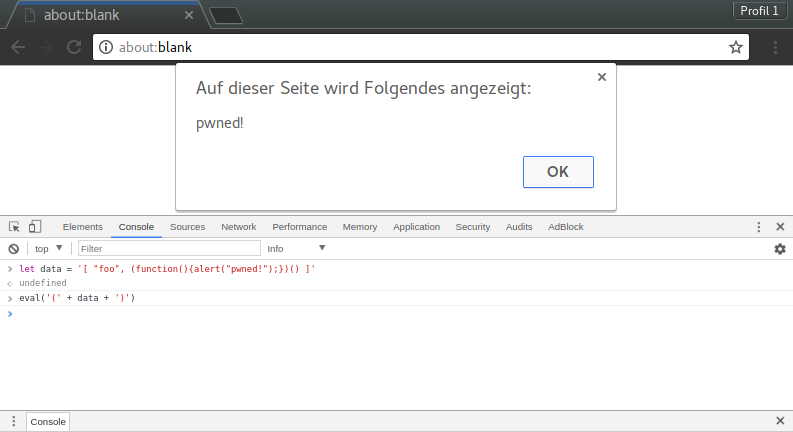
\includegraphics[width=\textwidth]{json-eval-alert}}
\end{center}
\caption{Der im String eingebetten Funktionsaufruf öffnet ein \mintinline{javascript}{alert()}-Benachrichtungsfenster im Browser.}
\end{example}
\end{figure}

Ein möglicher Angriffspunkt beim Einsatz von \acrshort{json}-verarbeitenden Applikationen auf JavaScript-Basis kann der Einsatz der \mintinline{javascript}{eval()}"~Funktion~\cite[Abschnitt 18.2.1]{ecma262} sein. Als Teilmenge von JavaScript\footnote{Auch wenn diese Aussage vom \acrshort{json}-Entwickler selbst stammt~\cite{crockford2006fatfree}, ist sie umstritten, da JavaScript auf Zahlen im IEEE-754 binary64-Format~\cite[Abschnitt 6.1.6]{ecma262} beschränkt ist. Im Gegensatz dazu enthält die \acrshort{json}-Spezifikation keinerlei Einschränkungen bezüglich der Fließkommagenauigkeit~\cite[Abschnitt 8]{ecma404} -- \acrshort{json}-Dokumente können daher auch Zahlen enthalten, die in JavaScript nicht darstellbar sind.} ist die Nutzung der Funktion zwar möglich, kann jedoch ohne weitergehende Validierung die Einschleusung von Schadcode ermöglichen.
